\subsection{Descrição do projeto}
Na primeira etapa do projeto, foi realizada a modelagem e analíse dos dados referentes a ligações recebidas por uma central de atendimentos.\\
Para isso, foram analísadas diferentes variáveis para que seu comportamento fosse análisado.\\
\begin{figure}[ht]
    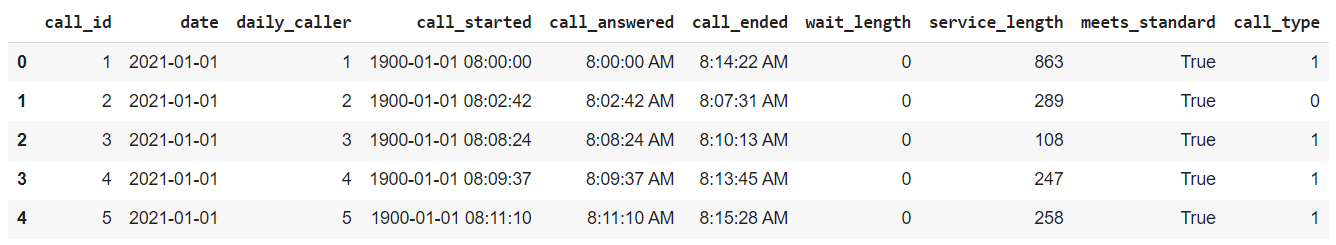
\includegraphics[scale= 0.6]{introducao/imgintro.png}
    \caption{Banco de dados - 5 primeiras chamadas}
    \label{fig: bd_img}
\end{figure}
Acima, pode-se observar 5 ligações registradas dentro da base de dados, bem como todas as variáveis. Call\_id é a identificação da ocorrência, date é a data, daily\_caller registra as ligações num dia, call\_started, call\_answered e call\_ended são os momentos de ligação, atendimento e término das chamadas. 
wait\_length é o tempo de espera,  service\_length é o tempo de atendimento, meets\_standard retorna verdadeiro caso o tempo de espera seja menor do que um minuto e call\_type é o tipo da ligação.\\
Para os testes de hipóteses atrelados às diferenças entre essas variáveis em diferentes períodos foi utilizado o método Kolmogorov-Smirnov para duas amostras que possui caráter não parametrico, sendo assim:\\
\begin{center}
$H{0}$ : Amostras seguem a mesma distribuição\\
$H{a}$ : Amostras seguem distribuições diferentes
\end{center}
Posteriormente a confirmação positiva da diferença entre amostras, foi realizado o teste de aderência das amostras às distribuições cauchy, chi quadrado, exponencial, gamma, lognormal, normal, powerlaw, rayleigh, uniforme.\\
Por último para analisar as correlações entre variáveis, foram realizadas regressões lineares e exponeciais.\\

\subsection{Próxima etapa}
Para a próxima etapa do processo, será realizada a modelagem da diferença entre chegadas (ligações) no sistema, para que posteriormente seja desenvolvida a simulação no ARENA.